\documentclass[10pt, conference, compsocconf]{IEEEtran}

\usepackage{capt-of}
\usepackage{graphicx}
\usepackage{subfig}
\usepackage{booktabs}
\usepackage{multirow}
\usepackage{siunitx}
\usepackage{multicol}
\usepackage{array}
\usepackage{amsmath}
\newcommand{\nltable}[2][c]{%
  \begin{tabular}[#1]{@{}c@{}}#2\end{tabular}}
\newcommand{\wave}{\raise.17ex\hbox{$\scriptstyle\mathtt{\sim}$}}

\newcolumntype{C}[1]{>{\centering\let\newline\\\arraybackslash}m{#1}}

\begin{document}
\bstctlcite{IEEEexample:BSTcontrol}

\title{Approach of Matrix Multiplication on Cloud Distributed System}


\author{\IEEEauthorblockN{Myungjun Son}
\IEEEauthorblockA{Department of Computer Science\\
Kookmin University\\
Seoul, South Korea\\
smj8612@kookmin.ac.kr}
\and
\IEEEauthorblockN{Kyungyong Lee}
\IEEEauthorblockA{Department of Computer Science\\
Kookmin University\\
Seoul, South Korea\\
leeky@kookmin.ac.kr}
}

% make the title area
\maketitle

\begin{abstract}
Cloud computing resources equipped with GPU devices are in wide usage because of extensive parallelism. They satisfy the demand for running data-mining applications which require the considerable amount of computing power by parallelism and enable users to save cost regarding money by renting the computing resources rather than acquiring physical ones.
    When running an application of Big Data in the cloud, people fail to know matrix computation is the key factor in determining the performance. Depending on some application and input size, the most time is used for data transfer for computation on GPU devices, and we cannot leverage cloud resources with GPU devices. Out of many resources by AWS EC2, there are some resources that can achieve better performance for matrix computation at a lower price than proposed resources from providers.
\end{abstract}

\IEEEpeerreviewmaketitle

\section{Introduction}\label{sec:intro}
Big data analytics systems are deployed in cloud computing environments to process ever-increasing dataset while guaranteeing stable operations; scalability and fault-tolerance from the perspective of infrastructure. To satisfy application demands from distinct use cases, cloud computing service providers offer various types of instances that the applications can run. For instance, a leading cloud computing service vendor, Amazon Web Services (AWS), provides over 60s of EC2 instance types that have unique hardware configurations\footnote{https://aws.amazon.com/ec2/instance-types/}. But, cloud platforms do not provide a clear methodology for exploring the configuration space.

Handling large-scale datasets require a massive amount of computing capacity, and most big data platforms are deployed in a scale-out manner. As managing distributed datasets and tasks running on large-scale machines can be challenging, abstractions of distributed datasets and resources are crucial to let application developers focus on tasks that matter. Many systems are proposed to provide a simple and easy interface to handle large-scale datasets, to name a few, Hadoop~\cite{hadoop}, Spark~\cite{spark}, and recently TensorFlow~\cite{tensorflow}.

However, the effectiveness of using cloud platforms and systems is highly dependent on the structure of input data and applications. In particular, matrix computation is dependent on the formation of input data in Spark. People fail to know what affects performance in each stage. For example, when doing matrix computation for small input matrices, gathering datasets from distributed platforms require less capacity. In this case, we can leverage instances that have a lower price than recommended ones from providers. 

We propose a solution to take a deep insight of main stages in Spark. We focus on what happens in the process of matrix computation in Spark and makes a model to let users have a better insight of choosing the structure of input data and optimal instances. 

The rest of the paper is organized as follows. Section 2 describes the process of matrix multiplication in a distributed system. Section 3 details overhead affecting in the process of computation and model with these overheads. Section 4 and Section 5 evaluates the change we propose and what can be learned from making models. Finally, in Section 6, we discuss related work and points out what is novel from them.



%big data processing engine including Spark, The importance of matrix multiplication
% change - various cloud computing resource configuration and difficult to find an optimal configuration
% mention the figure
% add overhead figure
% briefly mention other approaches to cover cloud configuration recommendation
% summarize proposed method
% summarize the result
% itemize the contributions
ddddddddddddddd
\begin{figure}[!ht]
  \centering
  \subfloat[Performance of different instance types of 2xlarge]{\label{fig:different-instance-types}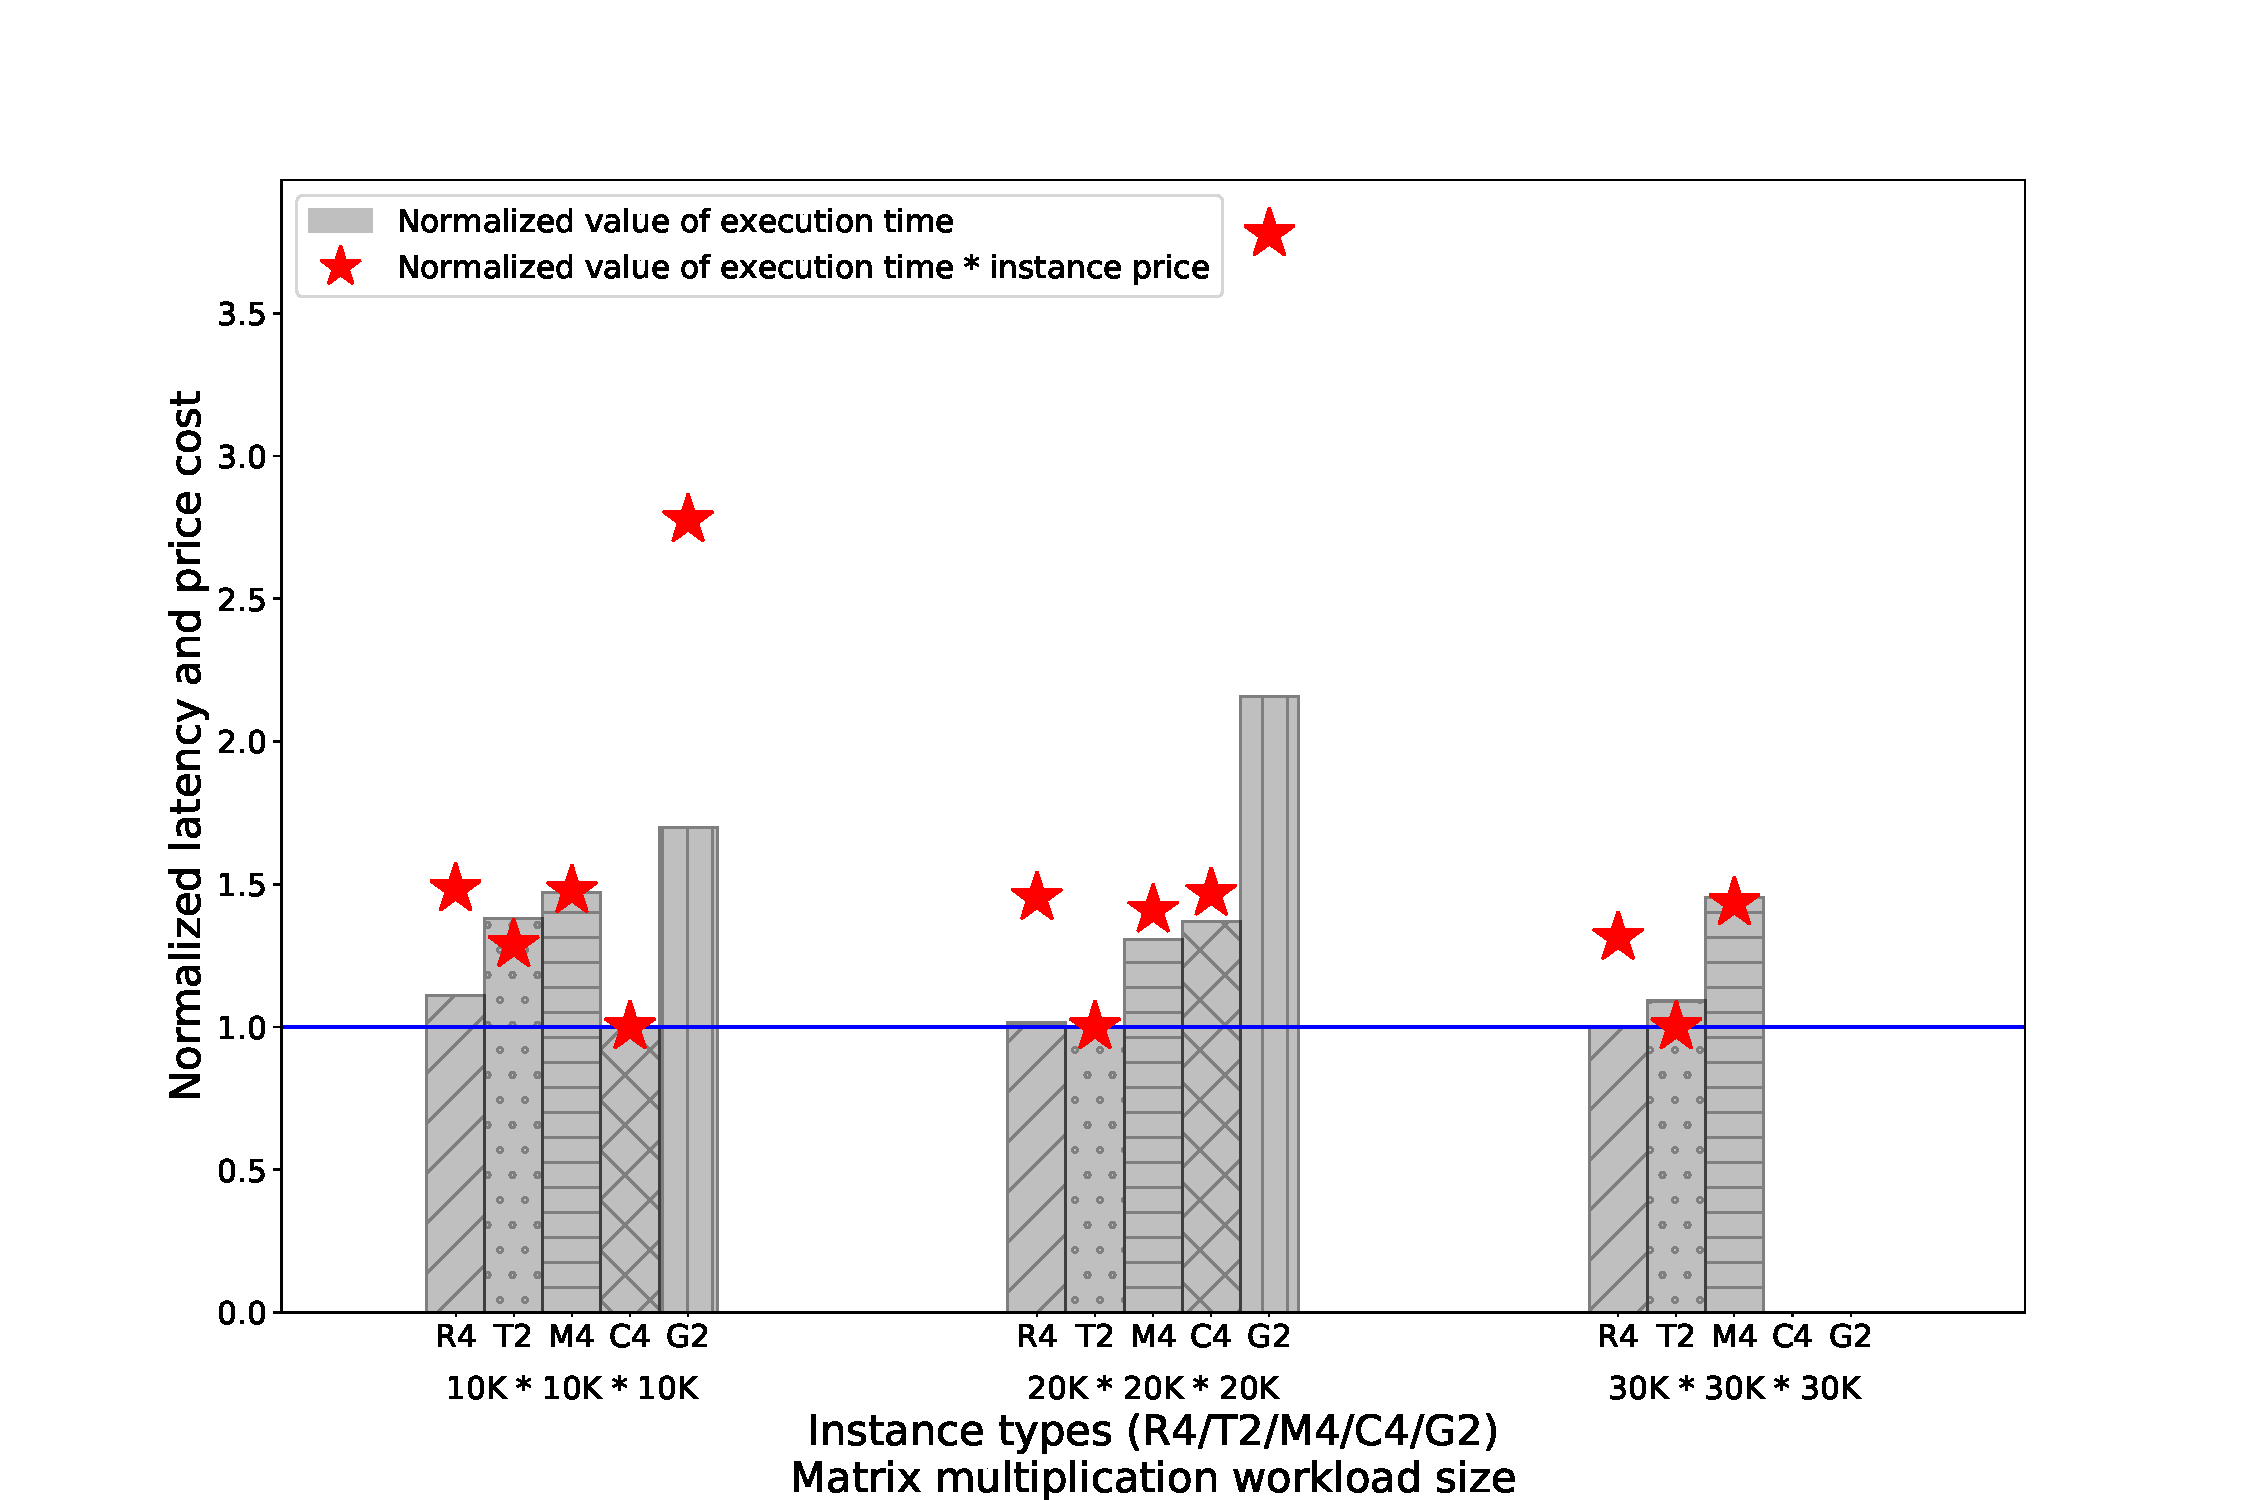
\includegraphics[width=0.5\textwidth]{figures/instance-2xl-compare.pdf}}\\
  \subfloat[Performance of different instance sizes of R4]{\label{fig:}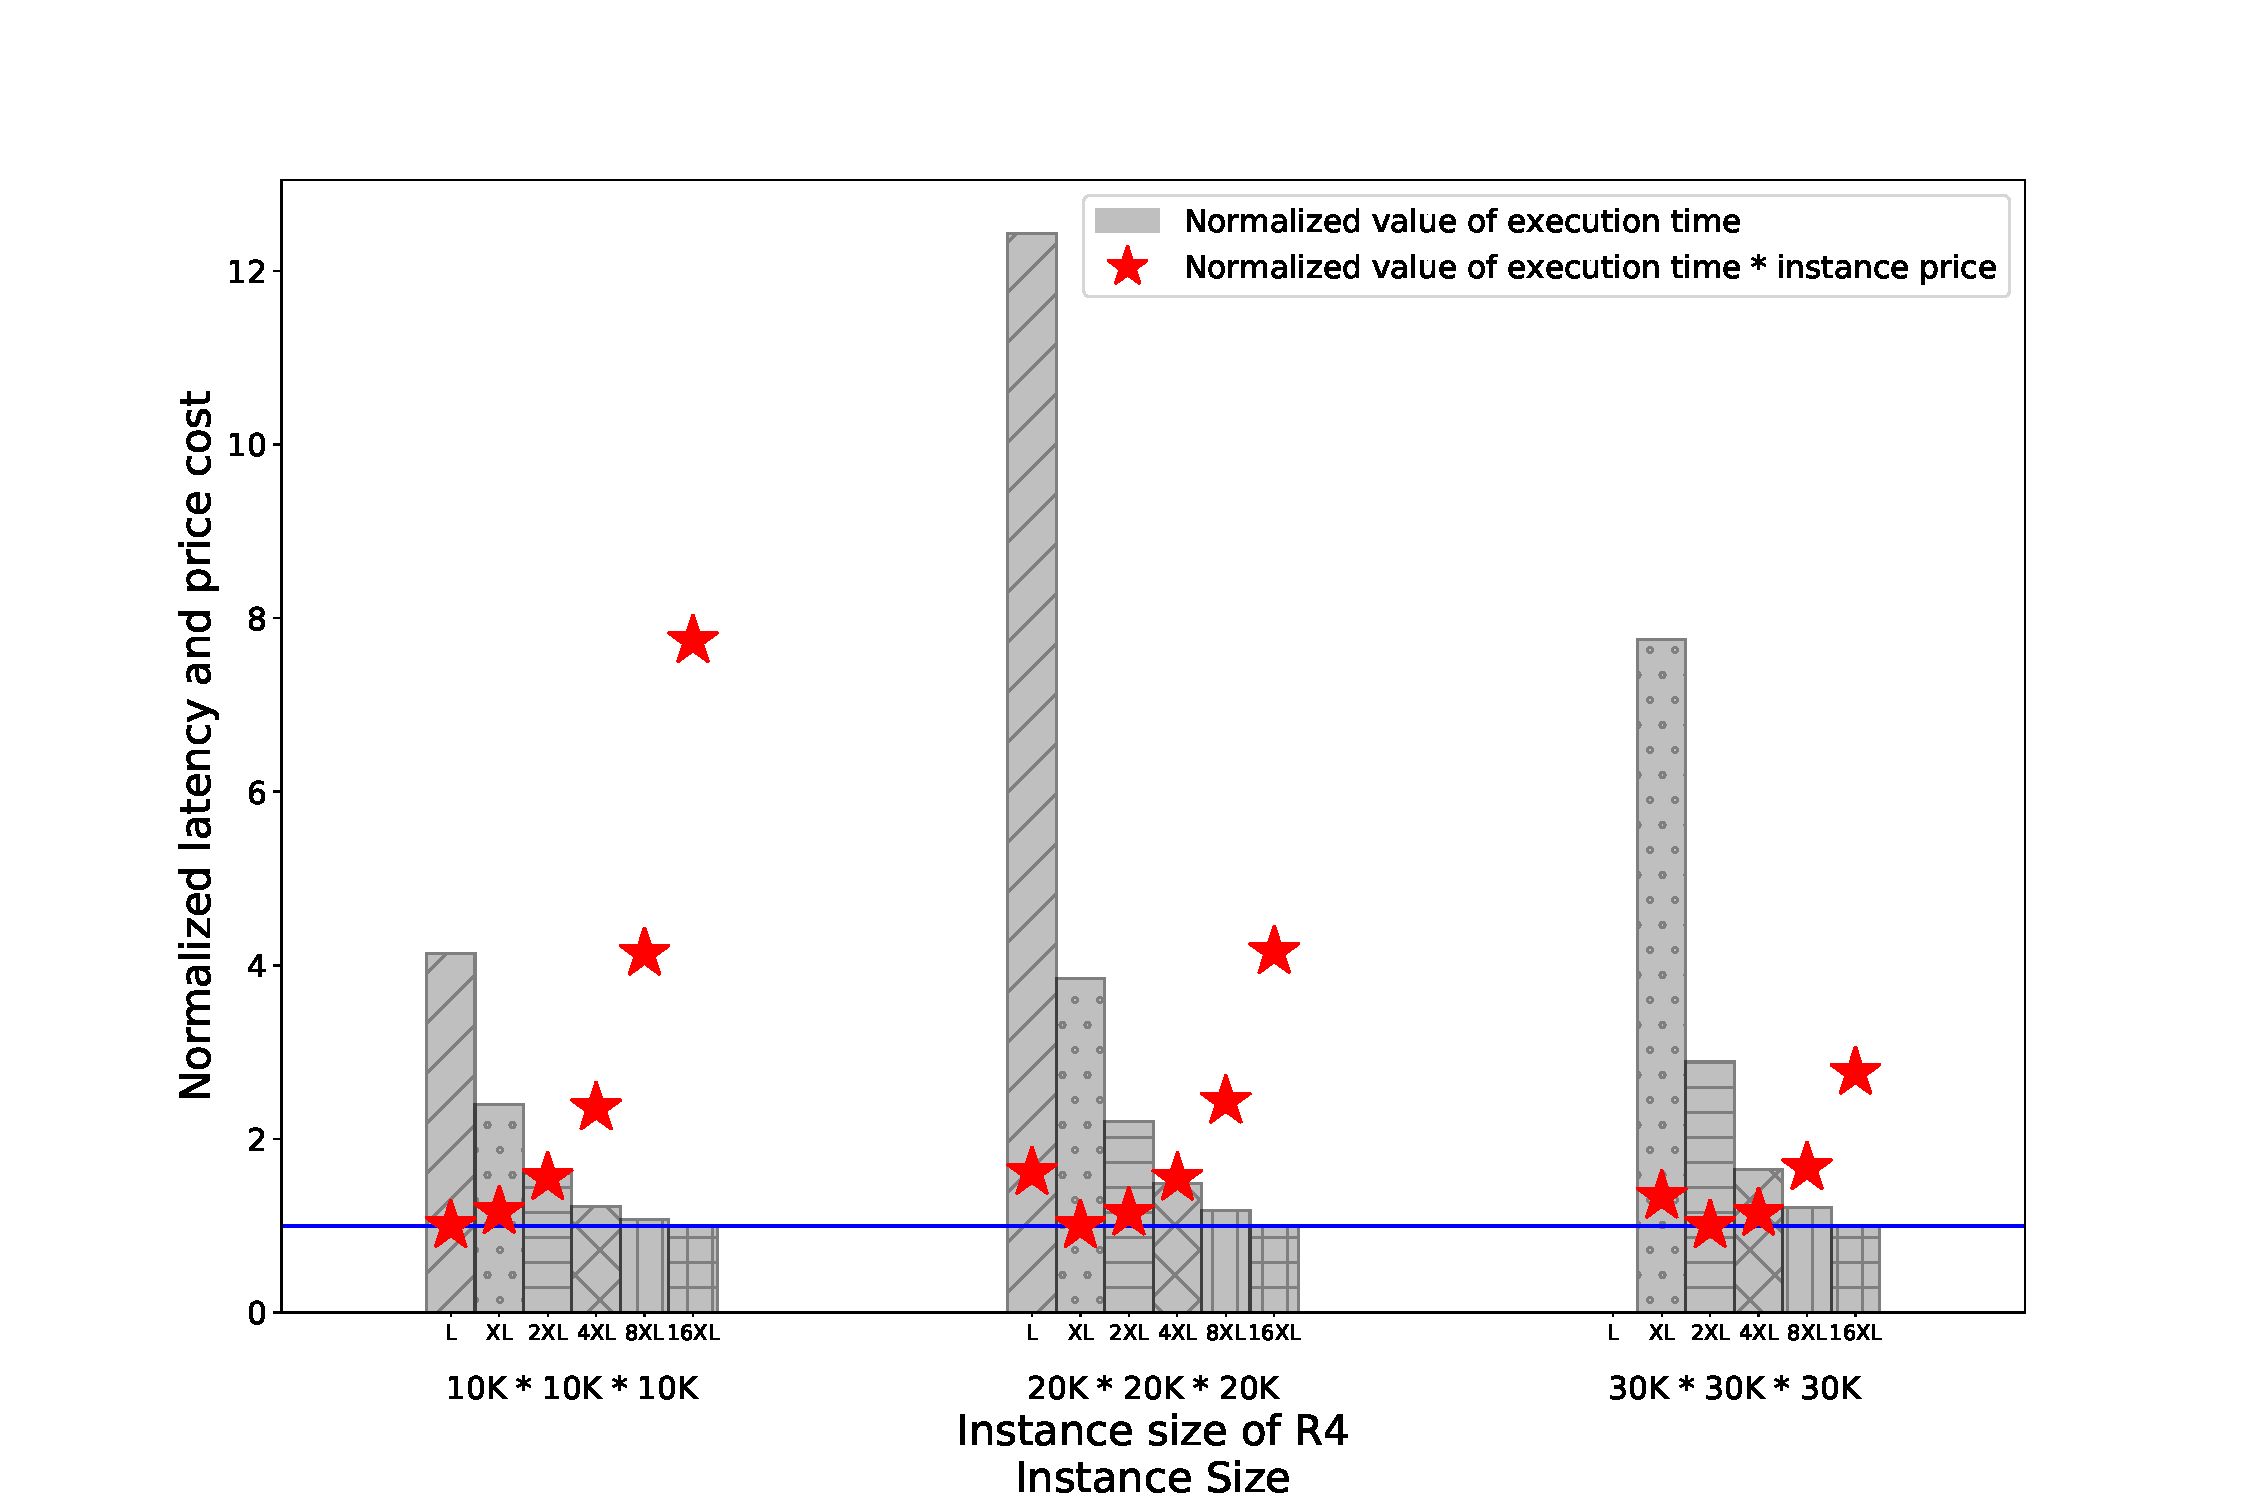
\includegraphics[width=0.5\textwidth]{figures/r4-sizes-compare.pdf}}
\caption{\label{fig:instance-blocks-sizes-compare}Comparision of various instance types and sizes to perform matrix multiplication of different sizes. The value shows the normalized value of latency and latency$\times$instance price - the lower, the better.}
\end{figure}

\section{Matrix Multiplication on a Distributed Computing Environment}\label{sec:distributed-matrix-computation}

% explain how the matrix computation happens in spark - mention the step of fetch, shuffle, compute, reduce
% plan to put 2 figures : 1 - local matrix & block matrix   2 - process of matrix multiplication with block matrix
% block matrix expression to be math expression

%%%%% To: MJ - need to mention row-, column-, and block- partition scheme


\begin{figure}[htp]
    \centering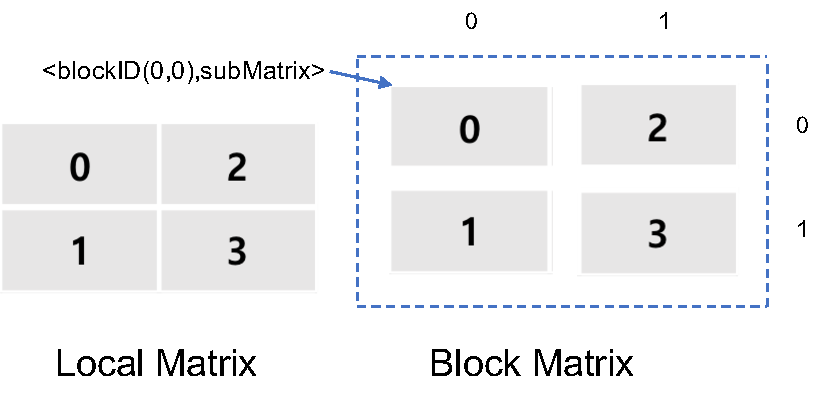
\includegraphics[width=0.4\textwidth]{figures/BlockMatrix.pdf}\caption{\label{fig:blockmatrix}Representation of Block Matrices}
\end{figure}

Apache Spark is a popular open-source platform for large-scale data. The primary abstraction in Spark is that of a resilient distributed
dataset(RDD), which represents a read-only collection of objects partitioned across a set of machines. Spark manages data using partitions that helps parallelize distributed data processing with minimal network traffic for sending data between executors~\cite{meng2016mllib}. Since Spark usually accesses distributed partitioned data, to optimize transformation operations, it creates partitions to hold the data chunks. 
   
In a matrix program on Spark, each matrix is associated with a partition scheme. Row/Column Scheme partitions the elements belonging to the same row/column into the same partition and each row/column is a local vector~\cite{yu2015exploiting}. Whereas, block partition scheme is splitting matrix into sets of sub-matrices. Block matrix treats the form as dense blocks of non-zeros, each block small enough to fit in memory on a single machine. In this paper, we consider block matrix because we focus on dense arrays and it has superiority when used in matrix multiplication rather than vectors. 

As shown in Figure ~\ref{fig:blockmatrix}, block matrix is represented as a key-value pair with the key denoting the block id and the value carrying the sub-matrix in the block. Each key-value is an element of an RDD. A block id is a wrapper over (block row, block column). We make use of block-splitting matrix multiplication, which splits two input matrices into blocked matrices and executes the sub-matrix multiplications in parallel across machines.~\cite{gu2015efficient}. On a single node, we use high-performance optimized linear algebra library, OpenBLAS~\cite{xianyi2014openblas}.

\begin{figure}
    
            \centering\subfloat[The Block-based distributed matrix multiplication on Spark ]{%
        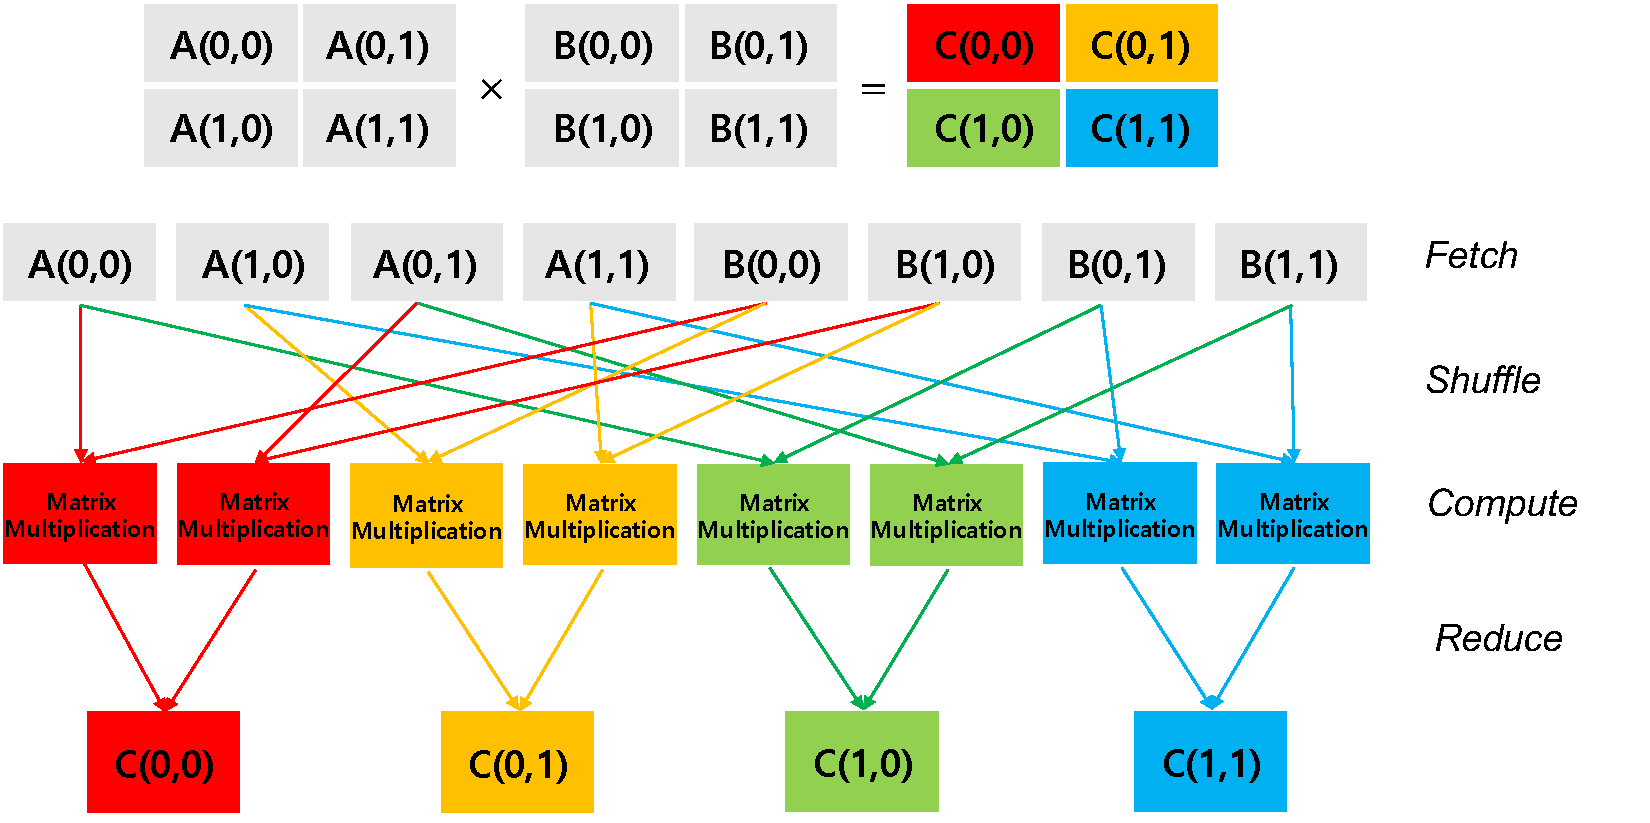
\includegraphics[clip,width=\columnwidth]{figures/MatMul.pdf}%
    \label{fig:matmul-whole}}

            \centering\subfloat[Overhead occurence per each stage]{%
    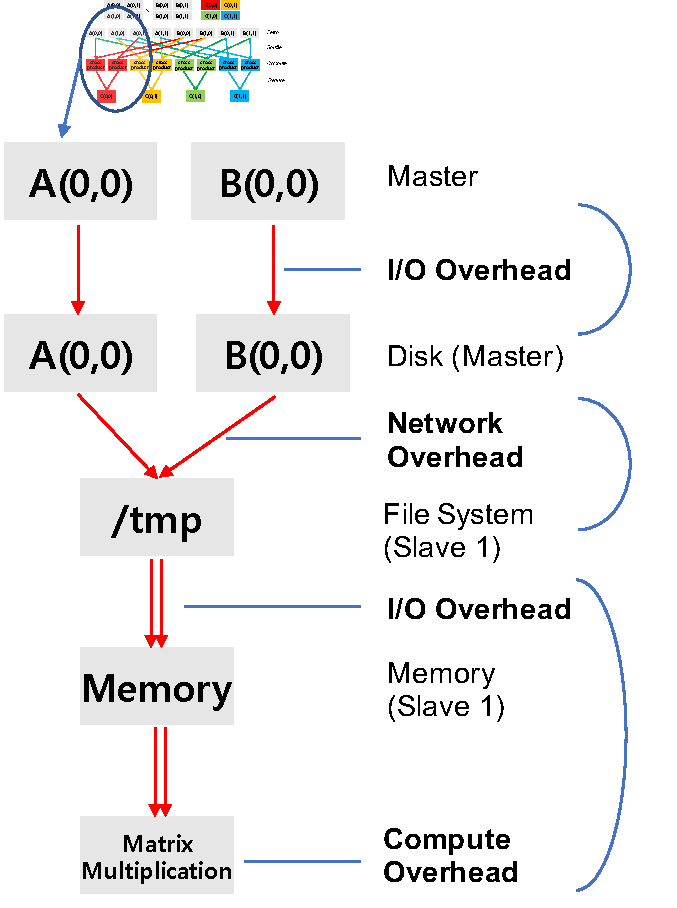
\includegraphics[clip,width=0.6\columnwidth]{figures/matmul-overhead.pdf}%
    \label{fig:matmul-overhead}}

    \caption{\label{fig:matmul}Block-based distributed matrix multiplication on Spark }
\end{figure}

As described in Figure~\ref{fig:matmul-whole}, the workflow of matrix multiplication can be mainly divided into 4 steps in terms of latency occurrence. In \textit{fetch} step, each input matrix is partitioned into $b\times b$ blocks, and each block is written to disk $b$ times which incurs \textbf{disk} overhead. this is related to flatmap(stage 6,7) in Spark. Spark predicts which block input matrices are needed to get each output block matrix. For example, from left input matrix A(0,0) is relevant to outputs of [C(0,0) , C(0,1)], A(0,1) is relevant to outputs of [C(0,0) , C(1,1)] , A(1,0) is relevant to outputs of [C(1,0) , C(1,1)], and A(1,1) is relevant to outputs of [C(1,0) , C(1,1)]. As a result, these block-matrices are written to disk $b$ times. 

In \textit{shuffle} step, the output of previous \textit{shuffle} step is transferred through the \textbf{network} in order to get related blocks together for the next step.

In \textit{compute} step, two related submatrices execute cross product locally using the native linear algebra library, OpenBLAS. this step is dependent on \textbf{clock rate}. After three steps, the last step is \textit{reduce} step gathering related cross product and summing these partial results together through \textbf{network}.

\section{Matrix Multiplication Overhead Modeling}
For a task of multiplication of two arbitrary size matrices, we analyze the overhead with a different number of available resources for the computation and unique formation of input matrices. For input left ($M_L$) and right ($M_R$) matrices, let us assume the number of rows of the left matrix is $r$, the number of columns of the right matrix as $c$. The number of columns of a left matrix and the number of rows of the right matrix is $k$. We denote the number of worker machines in a cluster as $n$.

On a distributed big data analytics engine, the degree of task parallelism is mainly dependent on the number of input matrix partitions and workers. In Apache Spark, the parallel execution of matrix multiplication task is achieved by dividing the output matrix to multiple blocks and computing each output block independently after fetching corresponding chunks from the left and right input matricies~\cite{spark-mm}. Deciding the optimal partitioning scheme of left, right, and output matrices with any number of resources are one of our on-going work. In this work, we focus on cases where the number of worker nodes is the squares of the arbitrary integer value, such as 1, 4, 9, etc. With this assumption, the input and output matrices are partitioned in a way that achieves the best parallelism, and this partitioning scheme is officially supported in the reference Spark matrix multiplication method~\cite{spark-mm-code}.

\subsection{Overhead Modeling with Different Number of Resources}\label{sec:overhead-number-of-nodes}
With $n$ worker nodes, where $n$ is a squared number of any arbitray number, to achieve the best parallelism, input and output matricies are block-partitioned (Section \ref{fig:blockmatrix}) that the dimension of left, right, and output blocks is $\sqrt{n} \times \sqrt{n}$. The number of elements in each block of the left matrix is $\frac{r \times k}{n}$, right matrix is $\frac{k \times c}{n}$, and the output matrix is $\frac{r \times c}{n}$.

With the above block-partitioned scheme, in the fetch and shuffle step, as we increase the number worker nodes, $n$, each block in the left and right matrices are required to be fetched and shuffled $\sqrt{n}$ times; the number of row/column blocks in the output matrix. As the size of each block is proportional to $\frac{1}{n}$, per worker fetch and shuffle overheads scale proportional to $\frac{1}{\sqrt{n}}$. With respect to the compute overhead, each output block that is assigned to a worker node needs to compute $\frac{r}{\sqrt{n}}\times k \times \frac{m}{\sqrt{n}}$. Thus, the compute overhead scales proportional to $\frac{1}{n}$.

In summary, in multiplying two matrices, increasing the number of worker nodes decreases the per-node fetch and shuffle overhead with the ratio of $\frac{1}{\sqrt{n}}$. The compute overhead decreases with the ratio of $\frac{1}{n}$. Note that the instance usage cost increases with the ratio of $n$.

\subsection{Overhead Modeling with Different Matrix Formation}\label{sec:overhead-non-square}
In distributed matrix multiplication performance modeling, it is essential to consider the effect of the parallel execution of independent tasks and block shuffling. For instance, the left and right fetch step in Figure~\ref{fig:matmul-overhead} happen in parallel as the tasks are not dependent on each other. It implies that the task scheduling and overhead of each fetch task can impact the overall task completion time. Furthermore, even in the computing step, the shuffled data read needs to be read from the temporary space (Spark local directory) that includes additional IO overheads. 

Given these features, matrix multiplication performance on Spark can be diverse depending on matrix input size and formation. In fetch step when two square matrices which have the same size are input for matrix computation, the task for each input matrix is executed parallel because they have the same size needed to be fetched incurring I/O overhead at the same time. I/O bandwidth is limited to Spark model which means doing fetch tasks parallel can have limited performance. Contrary to the square matrix in fetch step, non-square matrices, where left matrix doesn't have the same size as a right input matrix, latency is dependent on the bigger size of two. Because fetch step is blocking method for the next step, the smaller matrix is likely to be fetched earlier than bigger one and waiting. The bigger matrix then can fully use I/O bandwidth that leads to getting better performance on non-square matrices than square input matrices. In a thorough analysis, we found square matrices as input have more fetch latency that non-square matrices. This approach applies to compute step. To do the cross product, an executor has to wait for shuffled data to be read from Spark local directory, which is related to I/O overhead. In a square matrix, shuffled data get read parallel, but non-square matrices have different shuffled data size. The executor has to wait for the bigger input matrix size to finish reading the data which makes compute step latency longer. As can be seen in ~\ref{eval}. Evaluation section, although two input matrices size is same, a non-square matrix of the equal determinant had higher latency because of different two input matrices resulting in more time needed to read from the temporary space. Considering the formation of matrix and input matrix size is important.

% Mention how different formation (square, long-thin, wide-fat) have impact on each overhead

\section{Evaluation}{\label{eval}}

This section evaluates our overhead model in Spark. We run two tests: an experiment for evaluating overhead with a different number of resources and matrix formation, and for finding factors affecting overhead with different instance types. 
% show how our modeling method is precise (accurate)
\subsection{Experimental Setup}

We ran two tests on Amazon Cloud Compute clusters. For the first test, we used~\textit{r4.2xlarge} instances(details shown in Table ~\ref{table:r4.2xlarge} with various number of nodes. All nodes were located in the us-east-2 region (Oregon). We use Spark version 2.2.0 and Hadoop version 2.4.0 for HDFS and deploy on spark-ec2 tool, scripts used to setup a Spark cluster on EC2. OpenBLAS(CPU acceleration) was utilized for CPU acceleration

For second test, we used 21 instances (details shown in Table~\ref{table:experiment-configuration}) with 9 nodes. Rest of the experiment configuration is same as the one above test except ~\textit{g2} instance was using NVBLAS. For NVBLAS, we use the NVBLAS library shipped with CUDA toolkit 8.0.  

\begin{table}
  \caption{\label{table:experiment-configuration}Instance properties(Experiment 2)}
\begin{center}
    \begin{tabular}{ | l | l | p{2.0cm} |}
    \hline
    Instance Type & Min  & Max   \\ \hline
    C4 & LARGE & 8X.LARGE  \\ \hline
    R4 & LARGE & 16X.LARGE  \\ \hline
    M4 & LARGE & 16X.LARGE  \\\hline
    T2 & LARGE & 2X.LARGE   \\\hline
    G2 & 2X.LARGE & 2X.LARGE    \\\hline
    \end{tabular}
\end{center}

\end{table}

\begin{table}
  \caption{\label{table:r4.2xlarge}~\textit{r4.2xlarge} details}
\begin{center}
    \begin{tabular}{ | l | p{1.0cm} |}
    \hline
    Virtual Cores & 8   \\ \hline
    RAM & 61   \\ \hline
    Disks & EBS   \\ \hline
    Network & 10Gbps   \\\hline
    \end{tabular}
\end{center}
\end{table}

\subsection{Workload, Input matrix}

For a workload, we use general matrix multiplication kernel. This kernel is common among machine learning algorithms. When executing the matrix multiplication ten times for given input matrices in Spark, we took a close look at Spark between stage 6 and stage 9. We divided the calculation into three overhead stages as shown in Figure~\ref{fig:matmul}. For each stage, we collected task time on four nodes and chose the maximum values as latency for given input matrix overhead for each iteration. And out of values collected through 10 iterations, we set median value as a latency for the noisy data in cloud environments.

To show reliable support of overhead-based methodology, we select optimal data sets to cover arbitrary matrix size. We set the minimal row per block as 128 and maximum as 60000. Note that row/column per block size below 128 is excluded in the dataset because it makes no significant performance in any other instances. Starting from row size 128. We set matrix lengths as five levels: {minimum, low, central, high, maximum}. Using five degrees, we generated 15 input matrices. 

\subsection{Metrics}

need to mention about MSE, Sensitivity, 

\subsection{Experiment 1: Overhead with Different number of Nodes}

As mentioned in ~\ref{sec:overhead-number-of-nodes}, As the size of each block is proportional to $\frac{1}{n}$, per worker fetch and shuffle overheads scale proportional to $\frac{1}{\sqrt{n}}$. And the compute overhead scales proportional to $\frac{1}{n}$. Figure~\ref{table:15k-15k} shows the latency for 3 stages we stated according based on number of nodes for ~\textit{r4.2xlarge}. We can see the estimation similarly matches the actual performance. For example. When comparing fetch and shuffle latency for 16 nodes with nine nodes, those values increase to $\frac{3}{4}$.
For compute step, overheads increase to $\frac{9}{16}$. The reason shuffle latency for one node appears as $0$ is because all the computation is executed on a single node which doesn't need to gather results from a fetch step. 

\subsection{Experiment 2: Overhead with different matrix formation}

Matrix multiplication can be dependent on the structure of input matrices. ~\textit{fetch} and ~\textit{compute} step are related to disk overhead. To evaluate the section ~\ref{sec:overhead-non-square}, to examine the impact of the overhead performance, we ran three tests with four nodes. The results of this experiment are shown in Figures~\ref{fig:square-non-square}. We picked 60K * 0.1K * 30K as a baseline to compare with square matrices. From this input matrix, we can see left fetch overhead is similar to overhead from 2.7k * 2.7k * 2.7k. We ran dense matrix multiplication with square matrix above and measured the left fetch overhead. left fetch from non-square matrix had a lower value than that of square-matrix. For disk overhead and limited I/O bandwidth, the non-square matrix could avoid parallel disk write time for a period while left and right input matrix had to be fetched parallel. Right fetch step of square-matrix also showed higher values. 

For compute step, we picked 6k * 6k * 6k for input square-matrices which have same compute overhead as that of baseline(non-square) matrix. Seen from third and fourth bars, it is noticeable two latencies from compute step show big differences. The primary factor in this difference is, time used for moving datasets from local directory to memory. Within a square matrix, where the left and right matrices are fetched at the same time, most of the time is used for the cross product. However, CPU has to wait a long time for the bigger input(left input matrix) to execute the cross product which incurs long wait time. 


\subsection{Experiment 3: Scaling of input data}

With proposed model, to find out the performance change on the scaling of input-data size, we ran 2 tests on the same nodes. 
Table 3 presents the latency duration of each stage in both . The
configurations used in this experiment are as follows: all
Spark jobs are run on a 16-node m2.4xlarge cluster with
LZF compression enabled and the less compressible Workload. Table 
1.


% need to complete this part

% Metrics need to be used? (MSE)

\begin{table}

    \caption{\label{table:15k-15k}Latency for 15k * 15k * 15k (ms)}
    \centering
    \begin{tabular}{|C{0.7mm}| C{1.0cm}| C{1.1cm}|C{1.1cm}|C{1.1cm}|C{1.1cm}|}
        \hline
        \multicolumn{2}{|c|}{\multirow{2}{*}{}}&\multicolumn{4}{c|}{Number of Machines}\\
        \cline{3-6}
        \multicolumn{2}{|c|}{}&16 Nodes & 9 Nodes & 4 Nodes & 1 Node \\
        \hline
        \parbox[t]{2mm}{\multirow{3}{*}{\rotatebox[origin=c]{90}{Step}}}&Fetch& 1447.5&1931.5 &2844&5460 \\
        \cline{2-6}
        &Shuffle&887&947&1117.5&0 \\
        \cline{2-6}
        &Compute &7581.5&11543&22273.5&74513.3 \\
        %\cline{2-6}
        %&Asia &13.8(16.2)&27.5(47.0)&21.0(10.8)&10.2(11.7) \\
        \hline
    \end{tabular}

\end{table}

% things to show in Evaluation section
% 2. comparing 2k 2k 2k vs 128 60000k 30000k -> same block overhead, same computation time, but fetch overhead is different, I/O dominant 
% 3. latency for 3 stages decreases with increasing number of nodes from Table 1(still some exception)
% 4. median value on r4.2xlarge with 15 input matrix size cases with 3 different number of nodes -> can't figure out what to do with them 

\begin{figure}[htp]
	\centering
	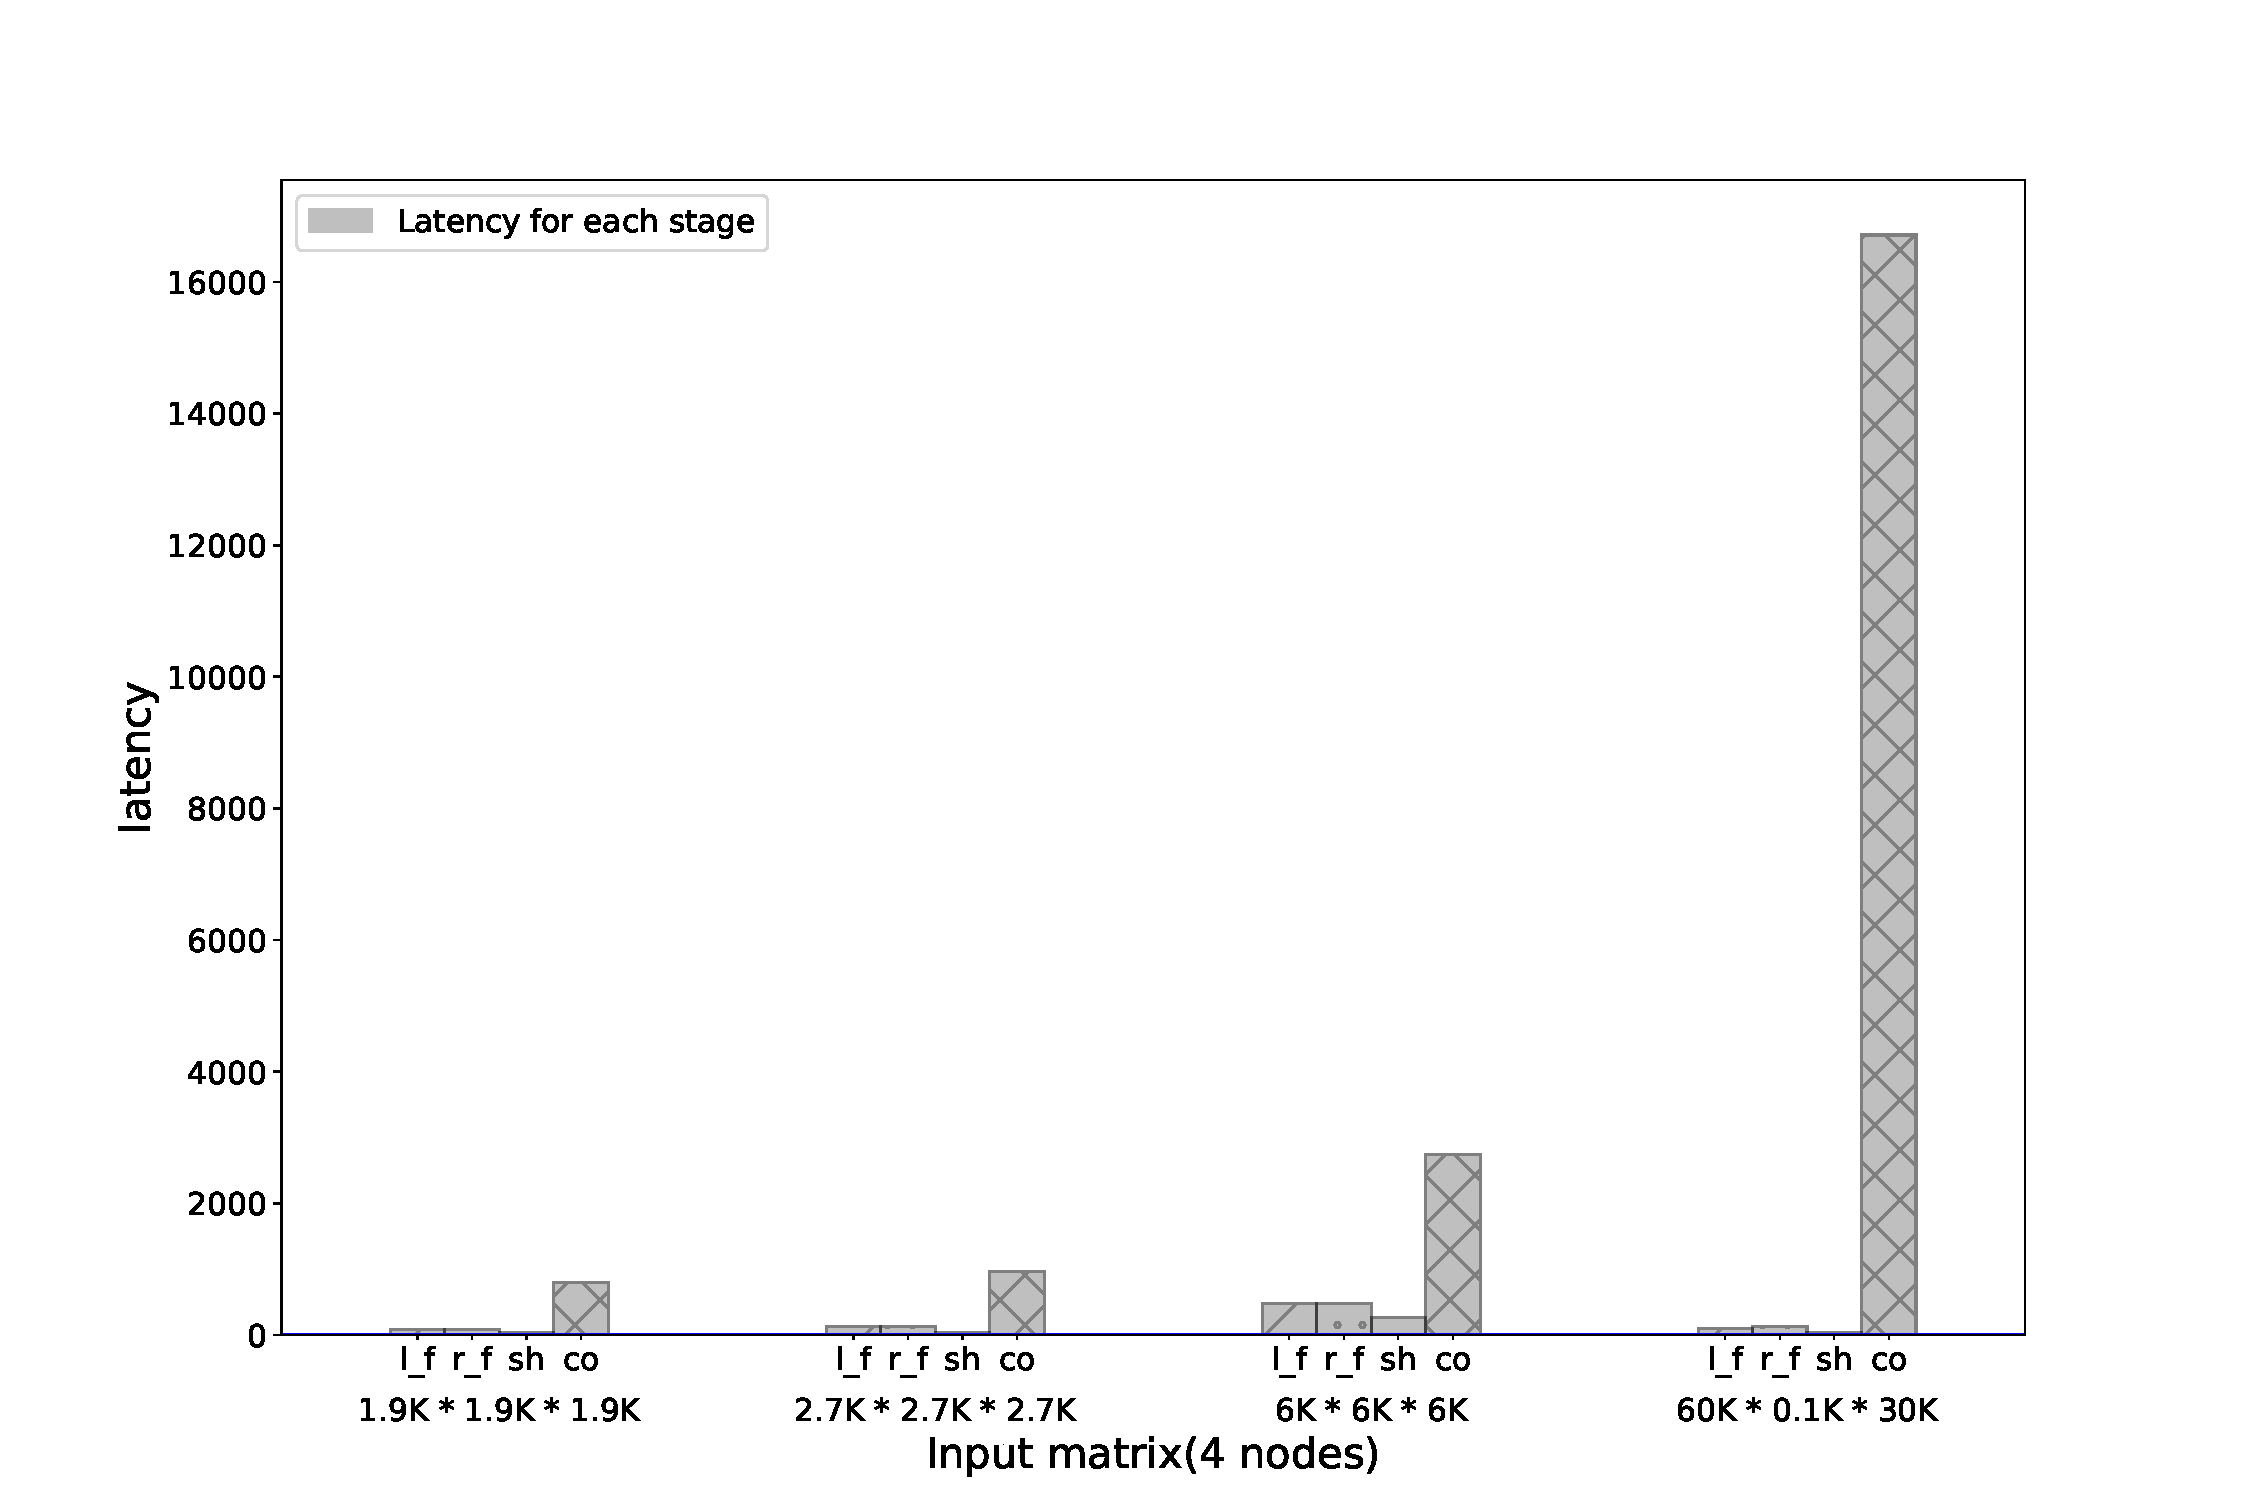
\includegraphics[width=0.4\textwidth]{figures/r4-2xl-square.pdf}\caption{\label{fig:square-non-square}Comparison with 60K * 0.1K * 30K}
	\captionof{table}[]{Latency duration for 4 input matrices }\label{tab:square-non-square-table}
% 	\centering
% 	\small
	\setlength\tabcolsep{5pt}
	\begin{tabular}{lcccc}
    \toprule
    \multirow{1}{*}{Input block size} &
      \multicolumn{1}{c}{l-fetch} &
      \multicolumn{1}{c}{r-fetch} &
      \multicolumn{1}{c}{shuffle } &
      \multicolumn{1}{c}{compute } \\
      \midrule
    ~\textit{1.9k * 1.9k * 1.9k} & 82.5 & 81.5 & 30.0 & 798.0  \\
    ~\textit{2.7k * 2.7k * 2.7k} & 129.5 & 129.5 & 44.0 & 960.5  \\
    ~\textit{3k * 3k * 3k} & 481.5 & 482.0 & 268.0 & 2744.5 \\
    ~\textit{60K * 0.1K * 30k} & 105.5 & 123.0 & 42.5 & 16713.0
    \\
    \bottomrule
  \end{tabular}
\end{figure}


\begin{figure}[htp]
	\centering
	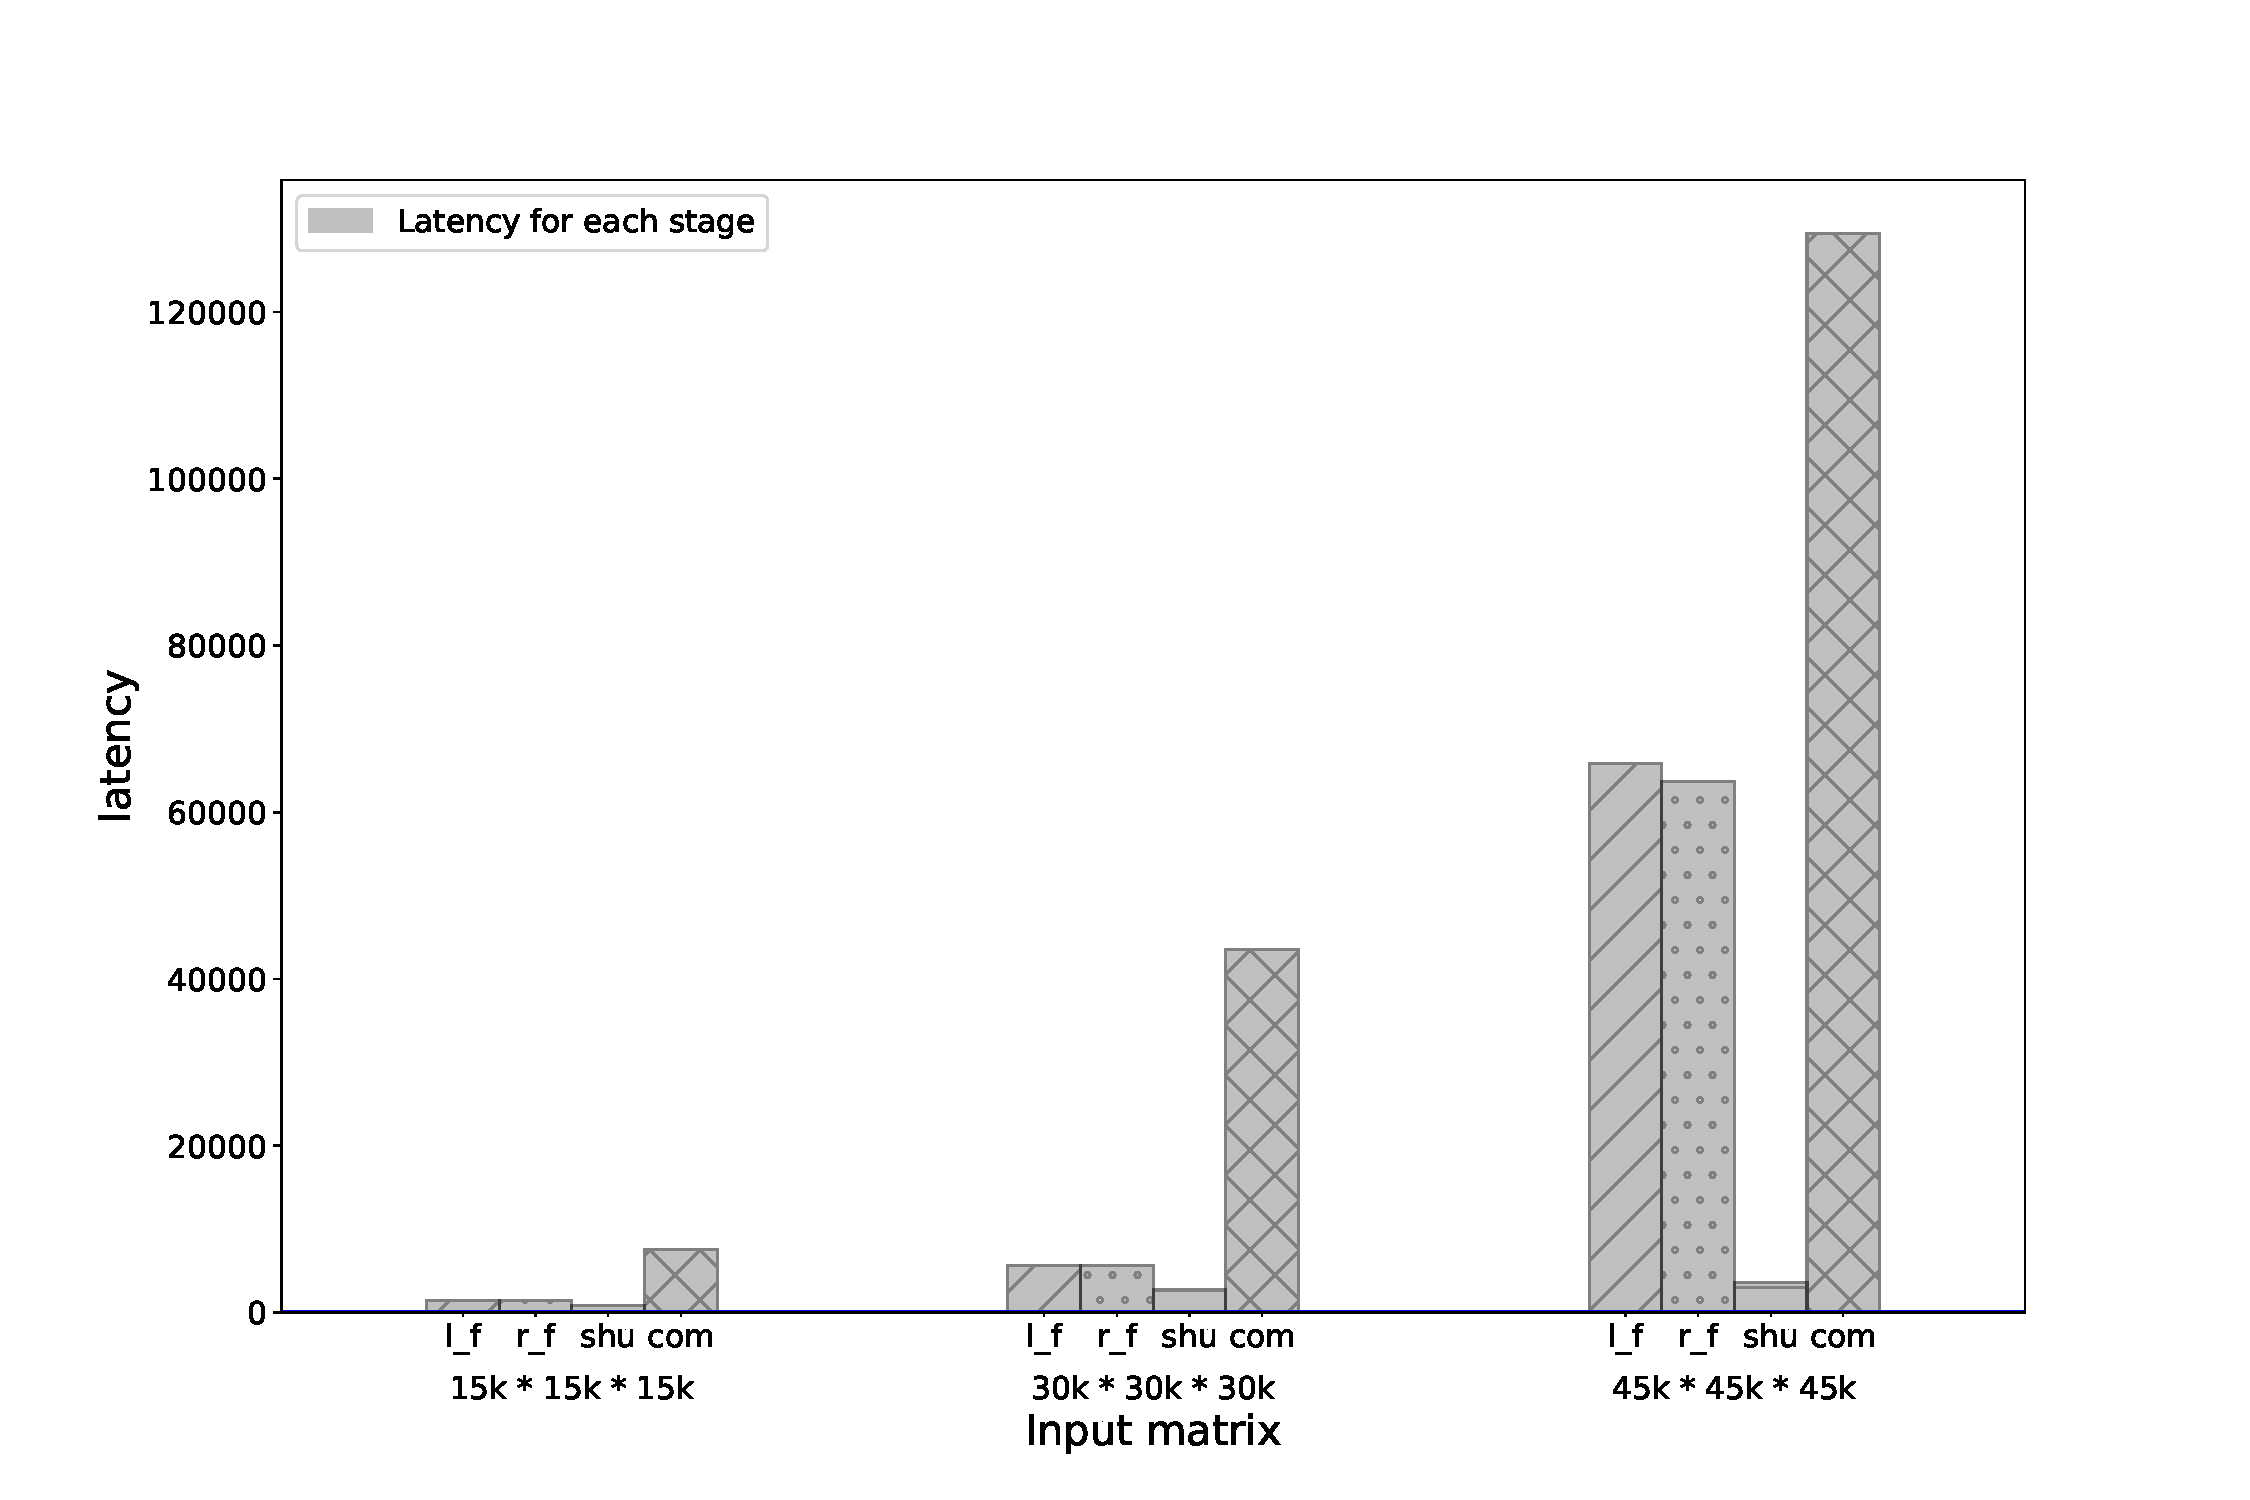
\includegraphics[width=0.4\textwidth]{figures/r4-2xl-square-scaling-16nodes.pdf}\caption{\label{fig:square-non-square}Comparison with square-matrix (16 nodes)}
	\captionof{table}[]{Latency duration for square matrices }\label{tab:square-non-square-table}
% 	\centering
% 	\small
	\setlength\tabcolsep{5pt}
	\begin{tabular}{lcccc}
    \toprule
    \multirow{1}{*}{Input block size} &
      \multicolumn{1}{c}{l-fetch} &
      \multicolumn{1}{c}{r-fetch} &
      \multicolumn{1}{c}{shuffle } &
      \multicolumn{1}{c}{compute } \\
      \midrule
    ~\textit{15k * 15k * 15k} &  1446.5 &  1447.5  & 887.0   & 7581.5 \\
    ~\textit{30k * 30k * 30k} &  5646.5 &  5631.0 & 2699.5  & 43568.0 \\
    ~\textit{45k * 45k * 45k} & 65787.5 & 63697.5 & 3572.0 & 129347.5\\
    \bottomrule
  \end{tabular}
\end{figure}


\section{Lessons Learned}
There are many instances supported by AWS. AWS recommends r4 instance as a recommendation instance for Spark. However, depending on the input size of the matrix, t2 type instances can achiever better performance at a lower price. Figure~\ref{fig:instance-blocks-sizes-compare} and Table ~\ref{tab:square-non-square-table} show that with input size 10k 10k 10k. T2.xlarge had the best performance compared to other general, GPU, memory-optimized instances. T2 type instances don't support hyper-threading compared to other instances. This feature can be useful for small input matrices. Likewise, although GPU instances may be good to use with large matrices on Spark, it is no good to use them with small matrices. We observed that up to block size of 32k * 32k *32k, using OpenBLAS outperformed NVBLAS(Spark equipped with cuBLAS)~\cite{nvidia2008cublas}. NVBLAS is a BLAS-3
library provided by NVIDIA built on top of cuBLAS-XT [2],
which supports a multi-GPU capable host interface. It's related to data transfer from/to CPU GPU for intensive computation which brings some overheads. Spark views machines as the collection of cores, and this could be another factor for the lower performance of GPU. 

Determining the right cloud configuration is quite challenging. Even if we focus only on performance based on overhead, the price of instance types remains non-trivial. Figure ~\ref{fig:instance-blocks-sizes-compare} compares the performance of the matrix multiplication of different using different sizes ~\textit{r4} instance type types converting the values to normalized ones. Seen from histograms on the table, three matrix multiplication performances benefit from the high size of the ~\textit{r4} instance type if we consider performance only. This result is not surprising because high instance size means more memory, CPU, etc. However, if we compare performance and cost of the instances together, results are peculiar. The red star indicates the normalized latency and price cost and the leftmost matrix multiplication performance is the best achieved by ~\textit{r4.l} instance. Instances have distinct prices which can make end-users more difficult to choose the optimal from different sizes of various instance types. The same applies to various types of instances. NVBLAS is a BLAS-3 library provided by NVIDIA built on top of cuBLAS-XT, which supports a multi-GPU capable host interface. In Figure~\ref{fig:different-instance-types}, it can be found that instances using OpenBLAS outperformed ~\textit{g2} instance using NVBLAS.  It's related to data transfer from/to CPU to GPU for intensive computation which brings some overheads. Spark views machines as the collection of cores, and this could be another factor for the lower performance of GPU.  
% OpenBla better than NVBLAS in experiment.
% Instance type (t2. g2, etc)
% Price consideration (latency is not the only metric)

\section{Related Work}\label{sec:relatedwork}
\textbf{Instance Recommendation:} Ernest~\cite{venkataraman2016ernest} predicts performance for different VM and cluster sizes, targeting machine learning analytics applications. PARIS~\cite{Yadwadkar:2017:SBV:3127479.3131614} takes a hybrid online/offline approach, using a random forest model to predict application performance on various VM configurations based on features such as CPU utilization obtained from profiling. None of these systems consider the I/O overhead modeling in distributed cloud environments with arbitrary matrix shape which can affect matrix computation performance. 

%need taming
\textbf{Analyzing performance of data analytics frameworks:} While previous studies have analyzed how CPU, memory, network and storage resources affect Spark performance ~\cite{196352,li2014tachyon,ousterhout2015making} our work is the first to take consideration that I/O overhead can affect shape of the matrix. 

dkfdkfjdkfj
% need taming
% cloud computing performance prediction
% instance recommendation (Ernest, Paris, CCGrid 2017)
% Matrix multiplication performance and Spark + Matrix multiplication

\section{Conclusion and Future Work}
Conclusion~\cite{tr-spark}


\bibliographystyle{IEEEtranS}
\bibliography{abc2}
\end{document}
